\chapter{Methodology}\label{chapter:methodology}

\begin{figure}
	\centering
	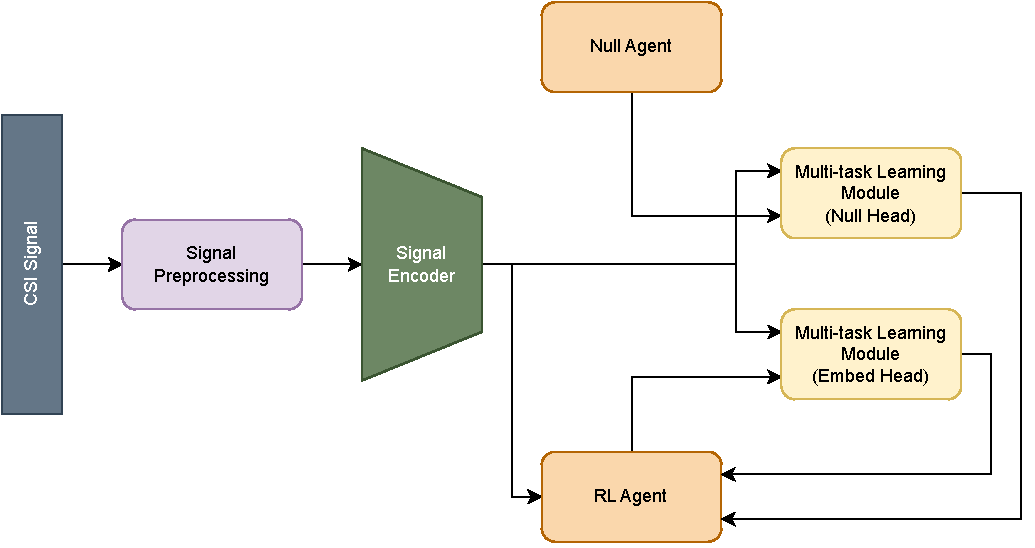
\includegraphics[width=\linewidth]{figures/arch_diagram.pdf}
	\caption{An abstracted diagram of the proposed DARLInG architecture.}
	\label{fig:arch-diagram}
\end{figure}

This chapter will first discuss the details of the dataset which we are using. 
We will discuss our approach to the problem of domain agnostic Wi-Fi CSI gesture classification and delve into the details of our chosen architecture.
This will first begin with a general overview of our method, then discuss each component of the architecture individually as well as their motivations and intuitions.

\section{Widar 3.0}

\begin{figure}
	\centering
	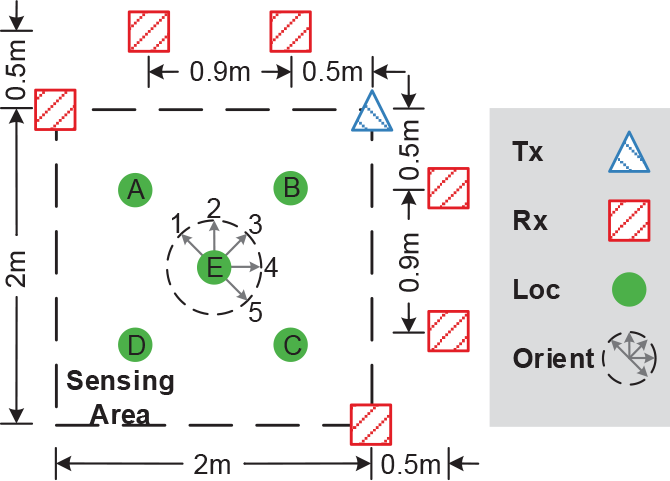
\includegraphics{figures/widar-positioning}
	\caption{Typical positioning of the access points and subjects in Widar 3.0. The image is sourced from \cite{zheng2019zero}. Loc shows the different torso locations used and orient the different orientations the subject may be at.}
	\label{fig:widar-positioning}
\end{figure}

The Widar 3.0 dataset \cite{zheng2019zero} contains gesture data collected over a series of months in 3 different rooms with 17 different subjects.
6 gestures were performed by every subject.
For each gesture performed, the gesture was performed in one of 8 locations with 5 orientations.
Further details of the distribution of domain factors can be found in Appendix \ref{appendix:dataset}.
Further details of how the data was gathered can be found in \cite{zheng2019zero}.

Each recorded data sample is a time-series consisting of the CSI between a transmitting Wi-Fi access point (Tx) and a receiving Wi-Fi access point (Rx).
Each Rx access point (AP) has two antennas, each of which are collecting separate time-series streams.
The positional setup of the gesture collection spaces can be seen in Figure \ref{fig:widar-positioning}.

The data itself is provided as a collection of both CSI data dumps, collected at 1000 Hz, as well as BVP tensors, collected with a temporal resolution of 10 Hz.
Each CSI data dump contains samples of sets of complex values with variable length, the shortest having a length of around 100 samples and the longest with a length of around 3100 samples. 
As the majority of the data have a length of less than 2000 samples, we set the cutoff to 2000 samples to ensure that every datapoint we use for training has the same length. 
We pad those of shorter length with 0s and we simply apply a cutoff on those datapoints which are longer.

Due to our focus on looking at single domain factor leave out as our main research question, we have chosen the task of single-user leave out.
To ensure that we are focusing only on this domain factor, our selection parameters for the training set and test set are seen in Table \ref{tab:single-user-select}.

\section{DARLInG}

In this thesis, we present our novel approach DARLInG (Domain Autolabeling through Reinforcement Learning for the Identification of Gestures).
DARLInG is our proposed approach to domain-agnostic gesture identification using RL.
Our intuition comes from \cite{zhang2021adversarial} in which RL was used to identify features in the data which was invariant to domain shifts.
Analogously, we hypothesize that RL can then be used to identify those features which are \textit{not} invariant to domain shifts and produce a \textit{domain embedding} from said features.
We hypothesize that by providing our gesture discriminator with not only the original signal, encoded by a VAE-style encoder, but also this domain embedding, the gesture discriminator would be able to significantly increase its performance in gesture recognition throughout multiple domains.

The general architecture of DARLInG can be seen in Figure \ref{fig:arch-diagram} and the code can be found publicly on GitHub\footnote{\href{https://github.com/yvan674/DARLInG}{https://github.com/yvan674/DARLInG}}.
We first propose a signal preprocessing and signal-to-image transformation pipeline, described in Section \ref{sec:methodology-signal-preprocessing} and \ref{sec:methodology-signal-to-image}.
This transforms the input signal into an image that is then passed through a CNN encoder, as described in Section \ref{sec:methodology-signal-encoding}, encoding the signal into a latent space.
This latent representation is then used in two different ways: As an input for the multi-task learning heads, described in Section \ref{sec:methodology-multi-task-learning}, and as the state observation for our RL agent, described in Section \ref{sec:methodology-rl}.

\begin{figure}
	\centering
	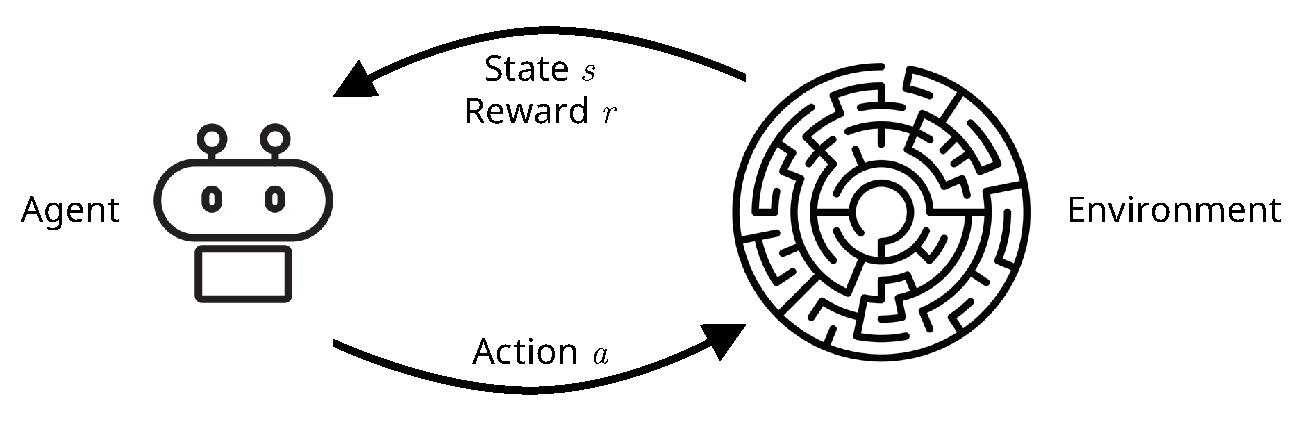
\includegraphics[width=0.78\textwidth]{figures/rl_paradigm}
	\caption{The basic paradigm of Reinforcement Learning where an agent interacts with its environment through actions $a$ and receives a new state $s$ and reward $r$ in return.}\label{fig:rl-paradigm}
\end{figure}
Recall first that RL is typically modeled as a Markov decision process with an environment and observed state of that environment at time $t$, $s_t$. An agent then performs an action $a_t$ and is provided with a reward $r_t$ and a new observed state $s_{t+1}$.
A typical RL scenario is framed in this way and is visually represented by Figure \ref{fig:rl-paradigm}.

To mitigate domain-shift, our RL agent is tasked with producing the best possible domain embedding of the domain $\boldsymbol{d}_r = a, \boldsymbol{d}_r \in [0, 1]^e$ as its action where $e$ is the dimensionality of the domain embedding.
The domain embedding, or action, is generated by the RL agent given the signal latent representation $\boldsymbol{z} = s, \boldsymbol{z} \in [0, 1]^f$ as its state observation, where $f$ is the dimensionality of the latent representation.

To provide the RL agent with a reward function, inspired by triplet loss, we use two different multi-task learning modules.
The details of the reward function are described in Subsection \ref{subsec:methodology-reward}.
One of these modules is provided $\boldsymbol{d}_{\emptyset}$, representing a vector of zeros when the $d$ is one-hot encoded or a value of $\frac{1}{f}$ when $\boldsymbol{d}_r$ is a probability measure, and the other $\boldsymbol{d}_{r}$.

\section{Signal Preprocessing}\label{sec:methodology-signal-preprocessing}

\begin{figure}
	\centering
	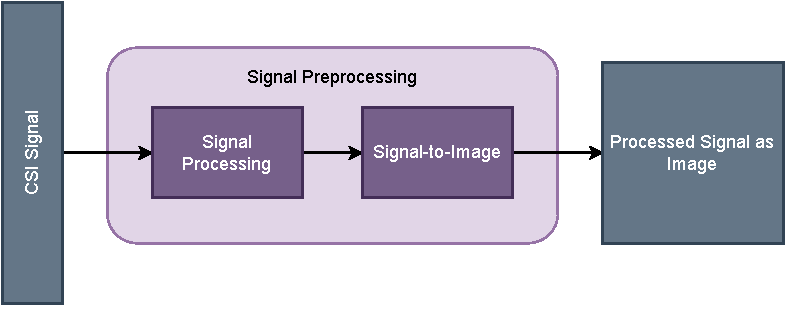
\includegraphics[width=0.8\linewidth]{figures/signal_preprocessing_diagram.pdf}
	\caption{Details of the signal preprocessing module. The module is comprised of traditional signal preprocessing and a signal-to-image transformation.}
	\label{fig:signal-preprocessing-diagram}
\end{figure}

As the old adage goes, garbage in, garbage out.
As such, we propose a signal preprocessing module, visualized in Figure \ref{fig:signal-preprocessing-diagram}.
This module first cleans the CSI signal using traditional signal processing and then transforms it into an image for use by the signal encoder.

\subsection{Signal Processing}

\begin{figure}
	\centering
	\begin{subfigure}{0.49\textwidth}
		\centering
		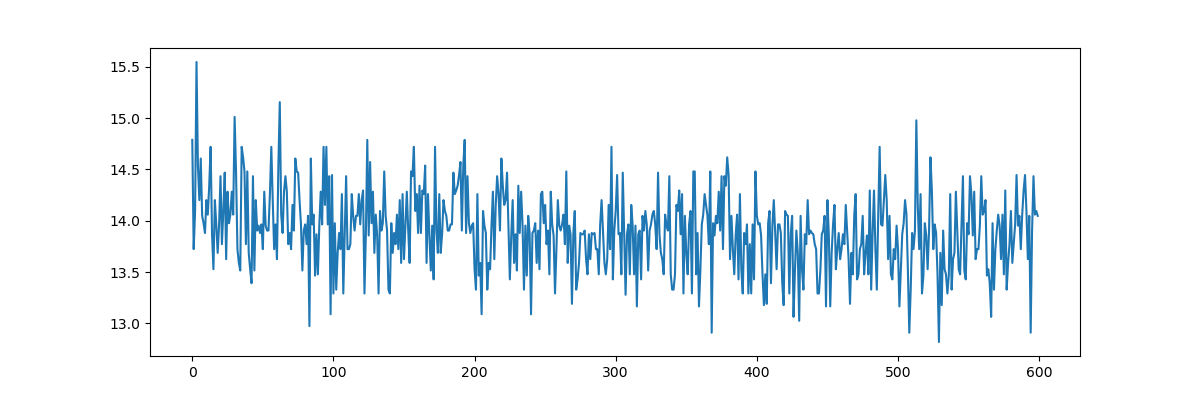
\includegraphics[width=\textwidth]{figures/amp_original}
		\caption{The original amplitude signal.}
	\end{subfigure}
	\hfill
	\begin{subfigure}{0.49\textwidth}
		\centering
		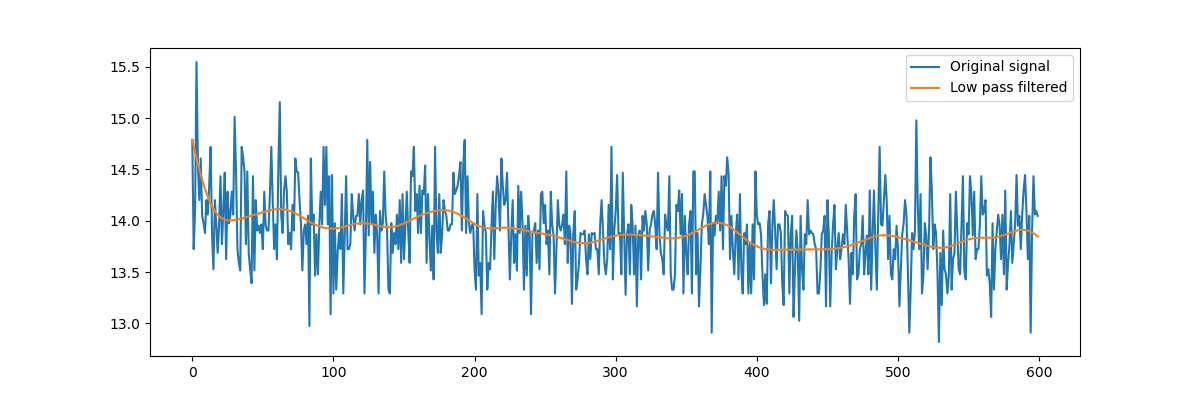
\includegraphics[width=\textwidth]{figures/amp_step_1}
		\caption{The original amplitude signal and the low pass filtered signal.}
	\end{subfigure}
	\hfill
	\begin{subfigure}{0.49\textwidth}
		\centering
		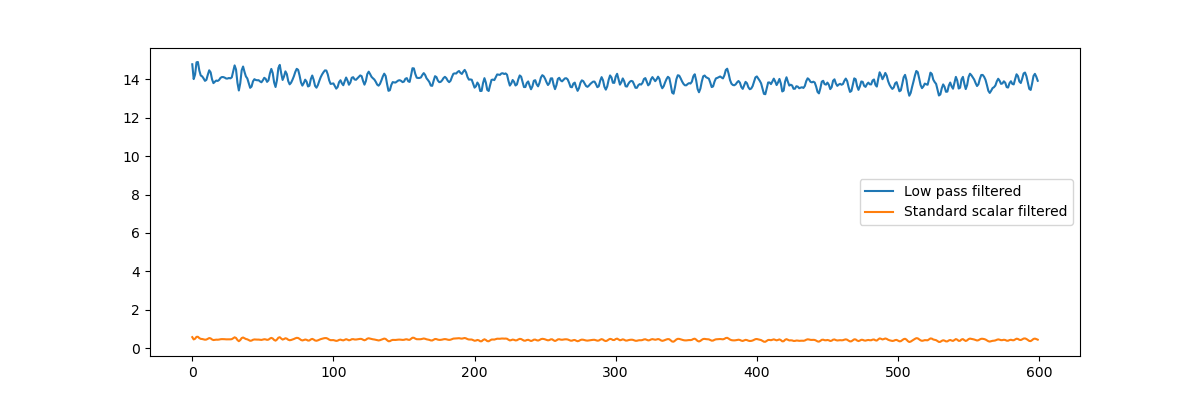
\includegraphics[width=\textwidth]{figures/amp_step_2}
		\caption{The low pass filtered signal and the signal after the standard scalar.}
	\end{subfigure}
	\hfill
	\caption{An example of the amplitude shift signal after being transformed by each step of the signal processing pipeline. Only the first 600 samples of one channel from one tranceiver link is shown here for illustrative purposes.} \label{fig:amp-pipeline}
\end{figure}

\begin{figure}
	\centering
	\begin{subfigure}{0.49\textwidth}
		\centering
		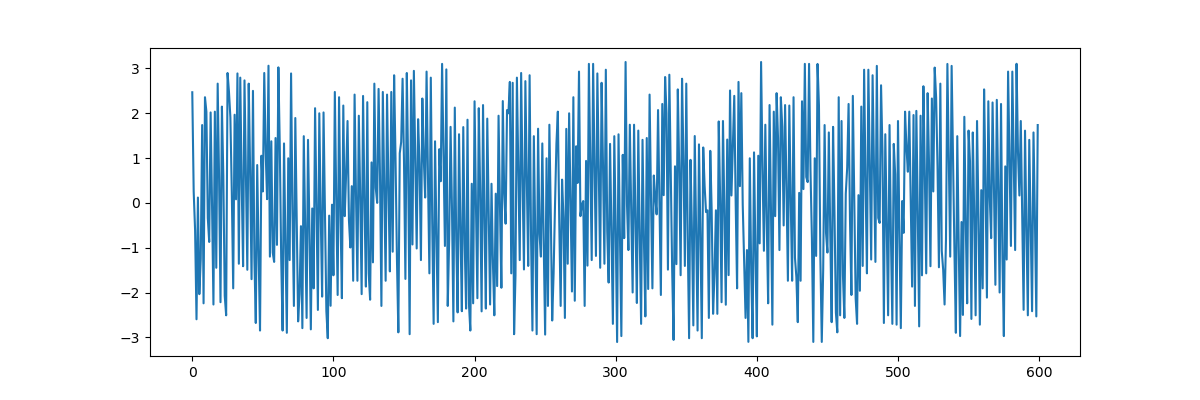
\includegraphics[width=\textwidth]{figures/phase_original}
		\caption{The original phase signal.}
	\end{subfigure}
	\hfill
	\begin{subfigure}{0.49\textwidth}
		\centering
		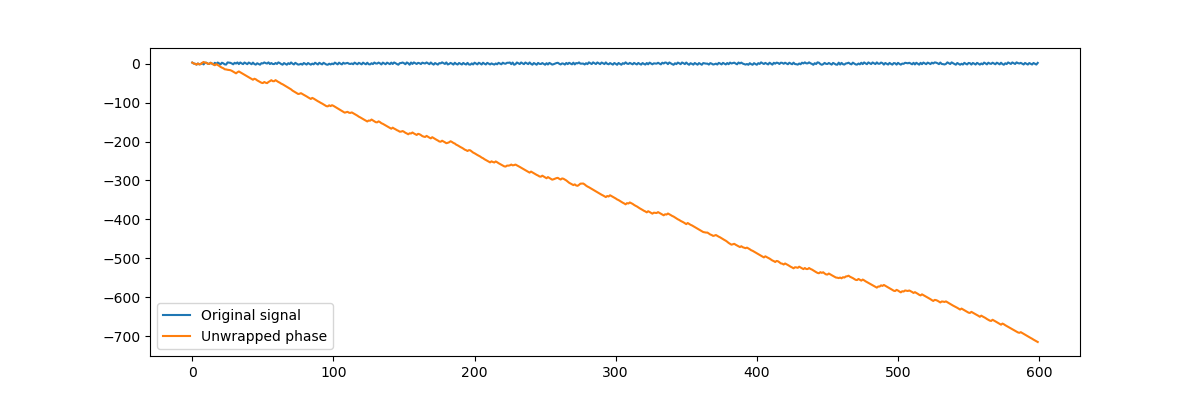
\includegraphics[width=\textwidth]{figures/phase_step_1}
		\caption{The original phase signal and the phase unwrapped signal.}
	\end{subfigure}
	\hfill
	\begin{subfigure}{0.49\textwidth}
		\centering
		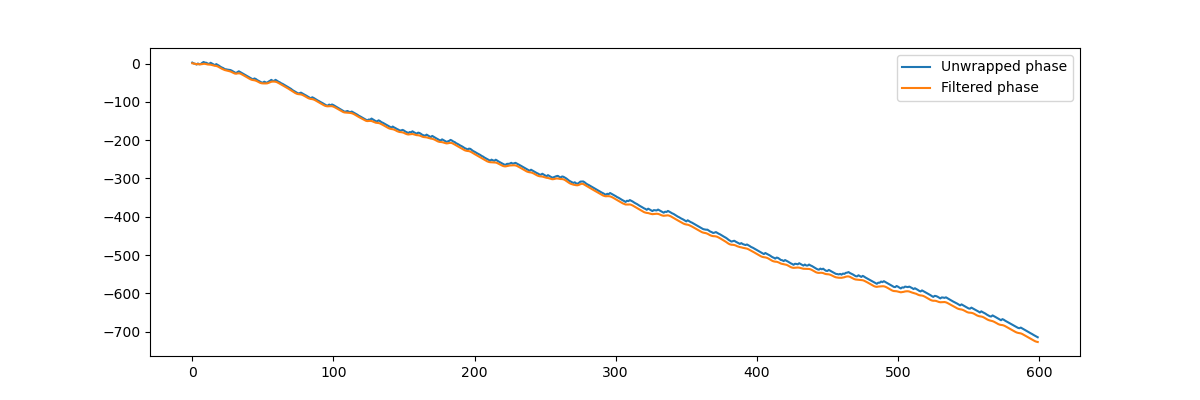
\includegraphics[width=\textwidth]{figures/phase_step_2}
		\caption{The phase unwrapped signal and the phase filtered signal.}
	\end{subfigure}
	\hfill
	\begin{subfigure}{0.49\textwidth}
		\centering
		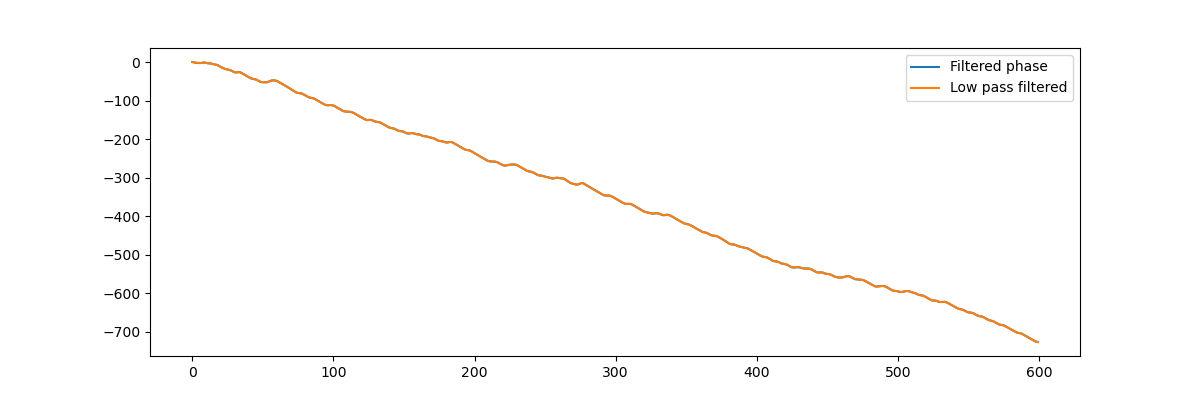
\includegraphics[width=\textwidth]{figures/phase_step_3}
		\caption{The phase filtered signal and the low pass filtered signal.}
	\end{subfigure}
	\hfill
	\begin{subfigure}{0.49\textwidth}
		\centering
		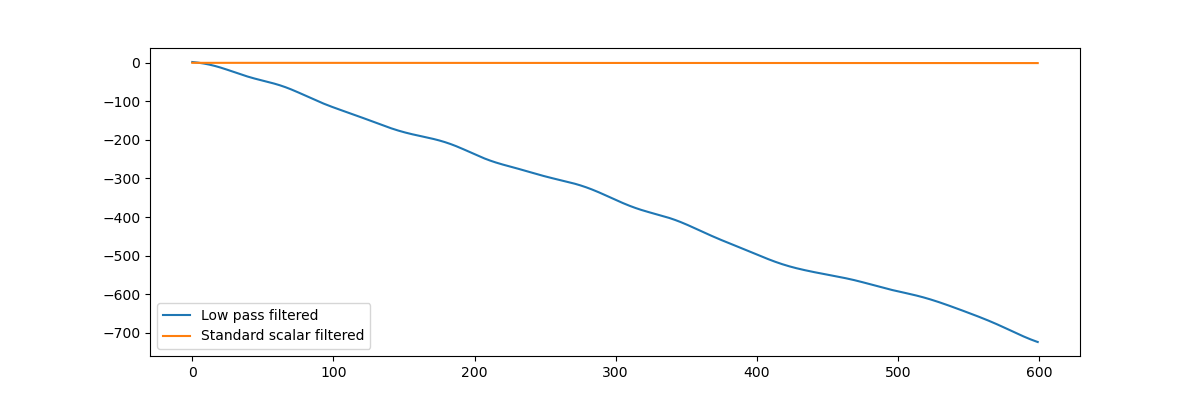
\includegraphics[width=\textwidth]{figures/phase_step_4}
		\caption{The low pass filtered signal and the signal after the standard scalar.}
	\end{subfigure}
	\hfill
	\caption{An example of the phase shift signal after being transformed by each step of the signal processing pipeline. Only the first 600 samples of one channel from one tranceiver link is shown here for illustrative purposes.} \label{fig:phase-pipeline}
\end{figure}

\begin{figure}
	\centering
	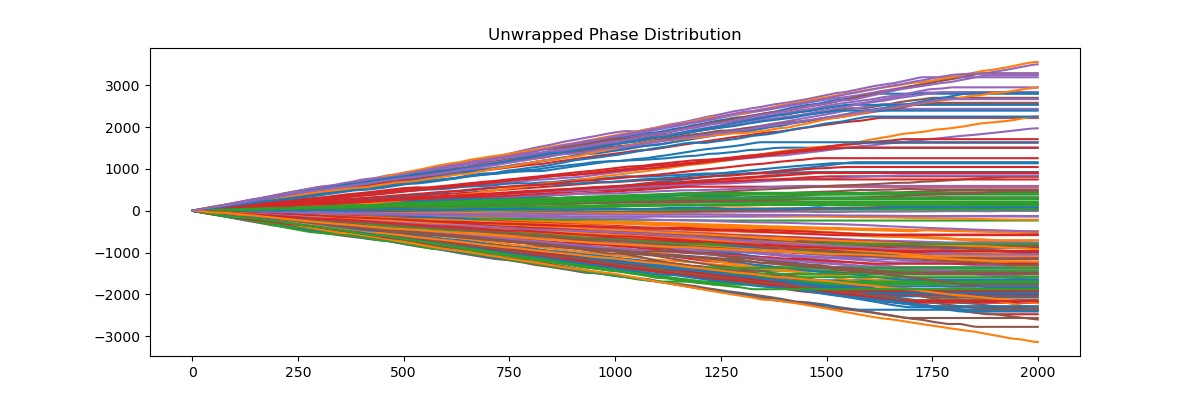
\includegraphics[width=0.8\textwidth]{figures/phase_unwrap}
	\caption{A plot over time of the phase shift after unwrapping of all training data, colored by gesture, showing how there is no general trend of only increasing or decreasing phases.}\label{fig:phase-unwrap}
\end{figure}

The CSI data is provided as a set of complex values sampled at 1000 Hz.
We first decompose this into its radius and angle components on the complex plane or its amplitude and phase shifts, respectively.
We process this signal through two different pipelines, one for the amplitude component and one for the phase component, as the phase requires a few additional processing steps compared to the amplitude.

The pipeline for amplitude consists of the following steps:

\begin{enumerate}
	\item \textbf{Low Pass Filter} set to a cutoff frequency of 250 Hz and an order of 4.
	\item \textbf{Standard Scalar} which has been trained on all training data and transforms the signal to have a mean of 0 and a standard deviation of 1.
\end{enumerate}

The low pass filter is used to eliminate noise inherent in CSI data from environmental factors.
It has also been set to these values based on empirical experimentation which shows that no human movements during the performance of the 6 gestures which we test for has a frequency above 250 Hz.

The standard scalar is used since empirical evidence shows that neural networks work best when input values are close to the interval $[-1, 1]$ \cite{varun2023tuning}.

The effect of each step of the amplitude pipeline can be seen in Figure \ref{fig:amp-pipeline}.

The pipeline for the phase consists of the following steps prepended to the amplitude pipeline:
\begin{enumerate}
	\item \textbf{Phase Unwrapping} which unwraps the phase and makes the signal continuous.
	\item \textbf{Phase Filtering} step, which applies a uniform and median filter onto the phase shift signal, inspired by \cite{oerlemans2022effect}.
\end{enumerate}

The effect of each step of the phase pipeline can be seen in Figure \ref{fig:phase-pipeline}.

The signal can now be considered clean, or at least clean enough that we can continue with further steps.

During the course of experimentation, we considered taking the derivative of the phase, to eliminate a generally monotonously increasing or decreasing signal, as can been seen in the example in \ref{fig:phase-pipeline} after phase unwrapping.
Further investigation showed that this is actually not necessary as most signals do not monotonously increase or decrease.
A plot of the phase shifts after unwrapping of all signals can be seen in Figure \ref{fig:phase-unwrap}.
The plot clearly shows that there is no general trend of phases increasing or decreasing infinitely, with many phase shifts staying around 0 after unwrapping.

\subsection{Signal-to-Image Transformation}\label{sec:methodology-signal-to-image}
\begin{figure}
	\centering
	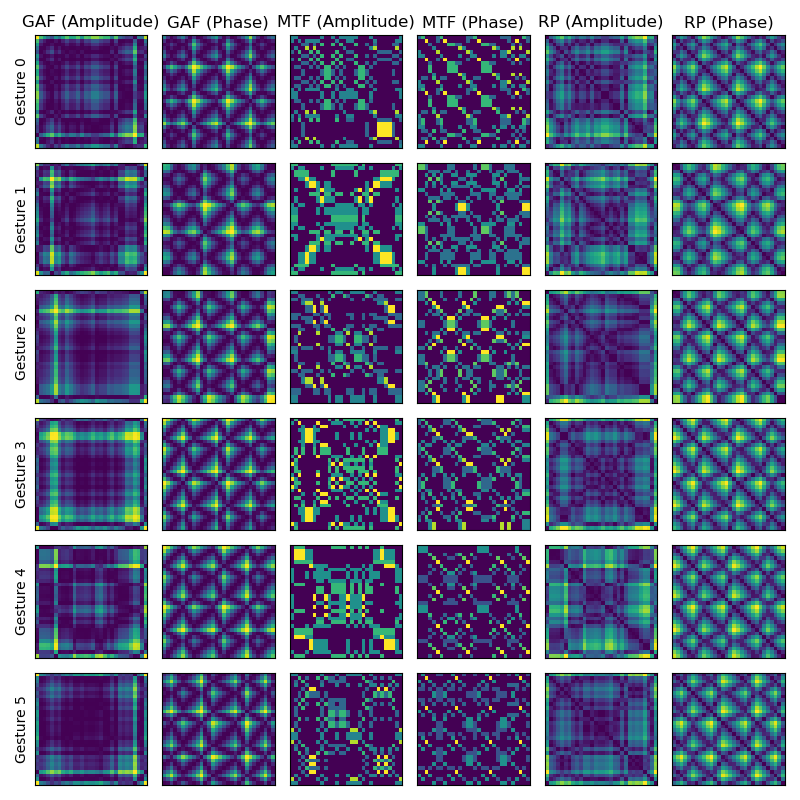
\includegraphics[width=\textwidth]{figures/transforms}
	\caption{Samples of each gesture from the Widar 3.0 dataset being transformed using each of the three signal-to-image transformations. Each pair of columns is the transformation by a single signal-to-image transformations on the amplitude and phase signals, respectively.}
	\label{fig:transform-samples}
\end{figure}

%Four crazy signal-to-image transformation methods! You won't believe number three!\todo{If there are no objections, this will be in the final paper}

The next stage in our method is transform the signal into an image, leveraging advances from computer vision.
There are many works from the literature which show that there are certainly improvements that can be gained from performing image processing on temporal data.
We will experiment with the following four methods for signal-to-image transformation: Gramian Angular Fields (GAF) \cite{wang2015imaging}, Markov Transition Fields (MTF) \cite{wang2015imaging}, and Recurrent Plots (RP) \cite{eckmann1995recurrence}.
A more comprehensive description of each of these transformations can be found in Section \ref{sec:background-signal-to-image}.

We process these images in Python using the pyts package \cite{faouzi2020pyts}, which conveniently contains ready-to-use implementations of all three of the aforementioned transformations.
Regardless of the chosen transformation, the signal is transformed into a two-dimensional tensor which can be treated as an image.
We also downsample this image to a size of $40 \times 40$ pixels for computational complexity purposes, which still provides a temporal resolution double that of the provided BVP data in Widar 3.0.
A visualization of each of the signal-to-image transformations on randomly selected samples of the Widar 3.0 dataset can be seen in Figure \ref{fig:transform-samples}.
As can be seen, each CSI sample is transformed into an amplitude as well as a phase image.
We can then proceed with the encoding of this image into a latent space.

\section{Signal encoding}\label{sec:methodology-signal-encoding}

\begin{figure}
	\centering
	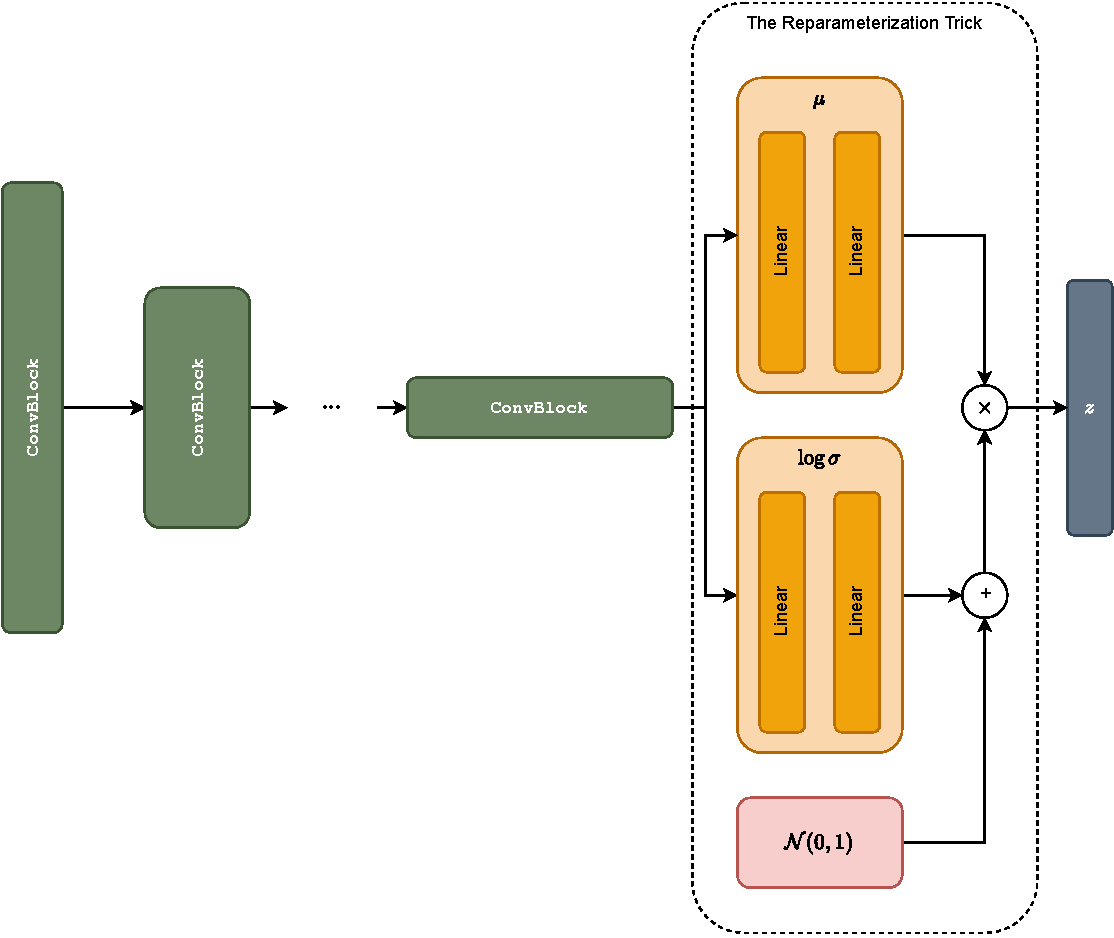
\includegraphics[width=\textwidth]{figures/vae-diagram}
	\caption{The CNN-based VAE used in DARLInG. The number of ConvBlock elements is variable, depending on the experiment being performed. The reparameterization trick is the same trick described in \cite{kingma2013auto}.}\label{fig:vae-diagram}
\end{figure}

The encoding of the signal, now an image, into a latent space is performed using a Convolutional Neural Network (CNN)-based VAE.
The CNN itself is structured as a standard, deep CNN, made up of multiple \verb|ConvBlock|s where each block is made up of a \verb|Conv2d| with dropout, a batch norm layer, and an activation layer.
The number of input channels, filters, and kernel size of the \verb|Conv2d| layer and its dropout is set dynamically and differs by experiment.
The activation layer also differs by experiments and is either ReLU, LeakyReLU, or SeLU.
The number of \verb|ConvBlock|s is set dynamically and differs by experiment.

These blocks are then followed by two sets of two fully connected layers with a hidden layer size of 8192.
One set of these fully connected layers serve to predict the $\mu$ of the other set to predict the $\log \sigma$ of the latent variables.
The reparameterization trick is then used, adding a random variable $\mathcal{N}(0, 1)$ to produce the latent variables $\boldsymbol{z}$.
A visualization of the CNN-based VAE used can be seen in Figure \ref{fig:vae-diagram}.

The latent representation $\boldsymbol{z}$ of this signal is then passed to both the reinforcement learning agent as its state observation as well as to the multi-task learning modules.

In the case of CSI data, as the signal is provided as both an amplitude and phase image, we have two signal-encoding modules running in parallel; one for the amplitude image and one for the phase image, with no sharing of parameters.
How the RL agent uses this state observation is described in Section \ref{sec:methodology-rl} while its use by the multi-task learning module is described in Section \ref{sec:methodology-multi-task-learning}.

\section{Multi-task Learning}\label{sec:methodology-multi-task-learning}

\begin{figure}
	\centering
	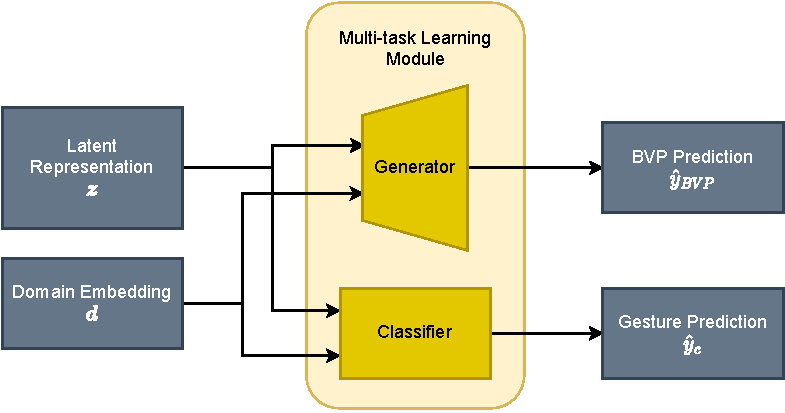
\includegraphics[width=0.8\linewidth]{figures/multitask_learning_module_diagram.pdf}
	\caption{Details of the multi-task learning module. The generator is made up of a series of deconvolutional layers and produces the BVP prediction while the classifier is a fully connected network and produces a probability distribution over each gesture class.}
	\label{fig:multitask-learning-module-diagram}
\end{figure}

The actual gesture classification module is built using a multi-task learning module, a visualization of which can be seen in Figure \ref{fig:multitask-learning-module-diagram}.
The idea, intuitively, is to enforce some sort of representation that is already approaching a domain-invariant representation of the data.
To do so, we use the generation of the BVP as an auxiliary task while keeping gesture recognition as our main task.
This is done as BVP is theoretically domain-independent \cite{zheng2019zero}, even though we are ultimately not interested in the BVP.
This approach is inspired by Martini et al. \cite{martini2021domain}, which, although using a different metric to modulate domain-independence as an optimization objective, suggests that an adversarial approach modulating both a domain-independence objective and a domain-discrimination objective can be powerful and increase classification performance.
The BVP generation is done by a series of deconvolutional layers while the classifier is a series of fully-connected layers.
Additionally, it has been shown empirically that multi-task learning can produce better results in each target task as opposed to dedicated networks \cite{tuggener2021deepscoresv2}.
This is likely due to the encoder being guided towards producing a more robust or efficient latent representation capable of being used for many different tasks instead of a latent representation focused on only one task.

Therefore, as BVP generation is a theoretically domain-independent process, we should expect the latent representation to contain both features which are completely domain independent as well as features which are not.
We do not, however, want to enforce domain-independence directly on the latent representation, as this may result in worse performance \cite{van2022insights}.
Further, \cite{martini2021domain} supports giving the latent representation domain-discriminatory powers.

As seen in Figure \ref{fig:arch-diagram}, we utilize two multi-task learning modules. The module receiving $\boldsymbol{d}_\emptyset$ is termed the \textit{null head} while the module receiving $\boldsymbol{d}_r$ is termed the \textit{embed head}. 
The motivation behind the use of two heads is such that we can measure the RL agent's performance in an unsupervised manner by comparing the performance of the null head to the embed head.
Intuitively, we should expect the embed head to perform better if the embedding $\boldsymbol{d}_r$ provided by the RL agent is able to provide some useful information, likely with respect to the domain, as opposed to the null head, which receives no useful information.
This comparison of the performance of the two embed heads is inspired by triplet loss.

For the loss function, we use cross entropy loss on the gesture classifier and mean squared error loss on the BVP generation.

\section{Reinforcement Learning Agent}\label{sec:methodology-rl}

To mitigate domain shift, we implement a novel method for unsupervised domain representations through reinforcement learning.
Recall the common terminology used in RL, the agent, the action $a$, the state observation $s$, and the reward $r$; and the learning paradigms discussed in Section \ref{sec:background-rl}.
For our agent, we choose to use the output of the encoder $\boldsymbol{z}$ as its state observation $s$.
The agent then performs an action $a$ which is what we refer to as the domain embedding $\boldsymbol{d}_r$.
This domain embedding is either continuous, in the case where the $\boldsymbol{d}_r$ is understood as a probability measure, or discrete, in the case where the $\boldsymbol{d}_r$ is understood as a one-hot encoding of domain factors.
The produced $\boldsymbol{d}_r$ is then concatenated to one copy of $\boldsymbol{z}$ and fed to the embed head, while the other head receives a copy of $\boldsymbol{z}$ concatenated with $\boldsymbol{d}_\emptyset$.
The reward $r$ is produced as a function of the outputs of both heads, and will be discussed further in Subsection \ref{subsec:methodology-reward}.

In this work, we will be looking at using both an on-policy and off-policy algorithm, PPO and DDPG, respectively.
Details of PPO can be found in Subsection \ref{subsec:background-ppo} while the details of DDPG can be found in Subsection \ref{subsec:background-ddpg}.
We use the ready-to-use implementation from Stable Baselines 3 \cite{raffin2021stable}, which also requires interpreting the model itself as a Gymnasium environment.
Gymnasium is an open-source RL framework previously mainted by OpenAI, but now actively maintained by the Farama Foundation \cite{towers2023gymnasium}.

Our use of RL to tackle this problem is inspired by both \cite{ma2021location} and \cite{zhang2021adversarial}.
In \cite{ma2021location}, as discussed in Section \ref{sec:literature-csi-for-gesture}, RL was successfully used to eliminate the need for domain-specific information Wi-Fi CSI gesture recognition.
On the other hand, as discussed in Section \ref{sec:literature-domain-rl}, \cite{zhang2021adversarial} used RL for domain-independent feature selection.
We therefore were motivated to investigate whether RL could also be used to perform the opposite: to extract relevant domain-specific features and produce a useful embedding of said features for gesture recognition.

\subsection{Reward Function}\label{subsec:methodology-reward}

As with any RL algorithm, one of the most important components is the reward function used.
We experiment with two different reward functions: One we call the \textit{contrastive reward} $R_{CON}$ and one we call \textit{distance-maximization contrastive reward} $R_{DMC}$.

\paragraph{Contrastive reward}
Let $\phi$ denote some metric subject to minimization to measure the gesture classification performance of a multi-task learning module given the gesture classification prediction $\hat{y_{c}}$.
The contrastive reward function $R_{CON}$ is then 
\begin{equation}
	R_{CON}(\hat{y}_{c,r}, \hat{y}_{c,\emptyset}, y_c, \gamma) = \gamma \cdot \left(\phi\left(\hat{y}_{c,\emptyset} - y_c\right(\phi\left(\hat{y}_{c,r}, y_c\right))\right)
\end{equation}
where $y_c$ is the ground truth gesture classification, $\hat{y}_{c,r} $ the predicted gesture from the embed head, $\hat{y}_{c,\emptyset}$ the predicted gesture from the null head, and $\gamma$ a multiplier factor chosen during hyperparameter tuning.
In practice, we use cross entropy loss as our performance metric $\phi$.
As such, our reward function $R_{CON}$ calculates the gesture recognition performance difference between the embed and null heads.

Intuitively, we use this as our metric as the reward is based on the performance difference between the two heads.
As the only difference in inputs between the two heads is that one receives $\boldsymbol{d}_r$ while the other receives $\boldsymbol{d}_\emptyset$, we should expect the difference in performance to come solely out of a difference in how powerful the domain embedding provided by the RL agent is in describing the domain factors influencing the CSI signal.
Thus, maximizing this difference implies better total model performance.
Additionally, we do not use an absolute value, as we want to penalize the model if the domain embedding results in the embed head performing worse than the null head.

This reward can be thought of as being similar to testing the null hypothesis, where $H_0$ is provided by the null head and $H_1$ is provided by the embed head.
Our hypothesis, that the domain embedding will provide better results, is measured by the performance difference between then null and embed head, by proxy.
If the RL agent provides a useful domain embedding, then the reward will approach $\gamma \cdot \phi\left(\hat{y}_{c,\emptyset}\right)$

\paragraph{Distance-Maximization Contrastive Reward}
Empirical results show that the contrastive reward was not able to produce good performance.
After inspecting the embeddings provided by our RL agent, we observed that the difference in value between each dimension was quite minimal, i.e., the agent produced results similar to $\boldsymbol{d}_\emptyset$.
We believe this is due to the agent attempting to minimize the penalty for worse performance without being incentivized enough to achieve positive rewards.

In response, we introduce our \textit{distance-maximization contrastive reward} $R_{DMC}$.
With this reward function, we hope to incentivize the agent to produce domain embeddings which are more informative by maximizing the difference between each dimension of the domain embedding.
The idea here is to provide stronger signals for the multi-task heads.
We do this by first calculating the pairwise difference between each of the dimensions.
We then apply a threshold to the difference, where any value below $\alpha$ is zeroed out, similarly to the procedure used in Lasso regression.
Finally, we sum together all differences and divide by the number of non-zero values and add the contrastive loss.
Formally, this can be described as
\begin{align}
	R_{DCM} (\hat{y}_{c,r}, \hat{y}_{c,\emptyset}, y_c, \boldsymbol{d}_r, \gamma) &= \gamma \cdot
		\frac{\sum_{i \leq e} \sum_{j \leq e, j > i} \left(|d_{r,i} - d_{r,j}|\right) \cdot \mathds{1}_{>\alpha}\left(|d_{r,i} - d_{r,j}|\right)}
		     {\sum_{i \leq e} \sum_{j \leq e, j > i} \mathds{1}_{>\alpha}\left(|d_{r,i} - d_{r,j}|\right)}
		+ R_{CON}(\hat{y}_{c,r}, \hat{y}_{c,\emptyset}, y_c) \\
	\text{where } \mathds{1}_A(x) &:= \begin{cases}
		1, & x \in A\\
		0, & x \notin A
	\end{cases},
\end{align}
$e$ the dimensionality of the domain embedding $\boldsymbol{d}_r$, $\mathds{1}_{A}(x)$ the characteristic indicator function, and $\alpha$ a hyperparameter to tune.
$d_{r,i}$ can be understood as the magnitude of the $i$-th dimension of the domain embedding
In practice, we set $\alpha = 0.1$.

\section{Model Training}\label{sec:methodology-training}

The general training process of the model is described in Algorithm \ref{algo:darling-training}.
We set the training of the RL agent to begin only at epoch $\zeta$ to ensure that the latent representation provided by the encoder has somewhat stabilized and actually contains useful information.
Otherwise, the RL agent will be training on garbage observation states.
This is especially relevant for DDPG, as the replay buffer may contain observations from those garbage environment states even during the later stages of training.
We alternate training between the RL agent and the VAE, rather than training both simultaneously, as we believe this will lead to more stable performance.

\begin{algorithm}
	\KwIn{Initialize parameters of the encoder $q$, the decoder of one multi-task learning module $p$, and the gesture classifier of one multi-task learning module $g$}
	\KwIn{$\zeta$, the epoch to begin phase 2 of training}
	\For{$k=0, 1, \ldots, N$}{
		\If{$k \geq \zeta$}{
			\If{$k=\zeta$}{
				Duplicate the multi-task learning module and its optimizer. The original multi-task learning module is designated the \textit{null head} and the new module the \textit{embed head}\;
				Initialize the RL agent\;
			}
			Freeze the parameters of the encoder $q$ and both the null and embed head\;
			Train the RL agent for $h$ epochs with samples from the training dataset, using the latent representation of a datapoint encoded by the encoder as a state observation\;
			Freeze the parameters of the RL agent\;
			Unfreeze the parameters of the encoder and both the null and embed heads\;
		}
		Train the encoder and all multi-task learning modules on the training set\;
	}
	\caption{Simplified DARLInG Training Algorithm}\label{algo:darling-training}
\end{algorithm}



